 
\section{Notation and Supporting Definitions}
\label{sec:notation}


In the following we start defining basic mathematical operations on integers and bit strings. From that we work our way to more specific basic methods used later in the specification.

\subsection{Data Types}

Bytes and byte strings are the fundamental data types. A byte is a sequence of eight bits. The set of bytes is denoted as $\byte$. A single byte is denoted as a pair of hexadecimal digits with a leading ``\texttt{0x}''. A byte string is an ordered sequence of zero or more bytes and is denoted as an ordered sequence of hexadecimal characters with a leading ``\texttt{0x}''. For example, \texttt{0xe534f0} is a byte string of length 3. An array of byte strings is an ordered, indexed set starting with index 0 in which all byte strings have identical length. We assume big-endian representation for any data types or structures.

\subsection{Functions}

We define the following functions:
\begin{description}
    \item[]$\lceil x \rceil$ (or $\funcfont{ceil}(x)$) for $x$ a real number returns the smallest integer greater than or equal to $x$.
    \item[]$\lfloor x \rfloor$ (or $\funcfont{floor}(x)$) for $x$ a real number returns the largest integer less than or equal to $x$.
    \item[]$\log(x)$ for $x$ a non-negative real number returns the logarithm to base 2 of $x$. In pseudocode this function is written as $\funcfont{lg}$.
    \item[]$\funcfont{Trunc}_\ell(x)$ truncates the bit-string $x$ to the first $\ell$ bits.
\end{description}

\subsection{Operations}

When $a$ and $b$ are integers, mathematical operators are defined as follows:

\begin{itemize}
    \item \^\ : $a^b$ denotes the result of $a$ raised to the power of $b$.
    
    \item $\cdot$ : $a\cdot b$ denotes the product of $a$ and $b$. This operator is sometimes omitted in the absence of ambiguity, as in usual mathematical notation.
    
    \item $/$ : $a/b$ denotes the quotient of $a$ by non-zero $b$.
    
    \item $\%$ : $a \% b$ denotes the non-negative remainder of the integer division of $a$ by $b$.
    
    \item $+$ : $a+b$ denotes the sum of $a$ and $b$.
    
    \item $-$ : $a-b$ denotes the difference of $a$ and $b$.
    
    \item $++$ : $a++$ denotes incrementing a by 1, i.e., $a = a + 1$.
    
    \item $<<$ : $a << b$ denotes a logical left shift of $a$ by $b$ positions, for $b$ being non-negative, i.e., $a \cdot 2^b$.
    
    \item $>>$ : $a >> b$ denotes a logical right shift of $a$ by $b$ positions, for $b$ being non-negative, i.e., $\funcfont{floor}(a/2^b)$.

\end{itemize}

The standard order of operations is used when evaluating arithmetic expressions.

Arrays are used in the common way, where the $i$-th element of an array $A$ is denoted $A[i]$. Byte strings are treated as arrays of bytes where necessary: If $X$ is a byte string, then $X[i]$ denotes its $i$-th byte, where $X[0]$ is the leftmost, highest order byte.

If $A$ and $B$ are byte strings of equal length, then:

\begin{itemize}
    \item $A$ AND $B$ denotes the bitwise logical conjunction operation.

    \item $A$ XOR $B$ (or $A \oplus B$) denotes the bitwise logical exclusive disjunction operation.
\end{itemize}

When $B$ is a byte and $i$ is an integer, then $B >> i$ denotes the logical right-shift by $i$ positions.

If $X$ is an $x$-byte string and $Y$ a y-byte string, then $X \| Y$ denotes the concatenation of $X$ and $Y$,with $X\|Y = X[0]...X[x-1] Y[0]...Y[y-1]$.

\subsection{Integer to Byte Conversion (Function \texttt{toByte})}

For $x$ and $y$ non-negative integers, we define $Z = {\tt toByte}(x,y) $ to be the $y$-byte string containing the binary representation of $x$ in big-endian byte-order.

\subsection{Member Functions (Functions \texttt{set, get})}

To simplify algorithm descriptions, we assume the existence of member functions. If a complex data structure like a public key $\pk$ contains a variable \texttt{X} then \pk.\texttt{getX()} returns the value of \texttt{X} for this public key. Accordingly, \pk.\texttt{setX(Y)} sets variable \texttt{X} in $\pk$ to the value held by \texttt{Y}. Since camelCase is used for member function names, a value \texttt{z} may be referred to as \texttt{Z} in the function name, e.g., \texttt{getZ}.

\subsection{Cryptographic (Hash) Function Families} 

\subsubsection{Tweakable Hash Functions (Functions \texttt{T, F, H})}

Following \SPHINCSP, a tweakable hash function takes a public seed $\pk.\seed$ and an address \ADRS in addition to the message input. This effectively renders hash function calls for each key pair and position in the virtual tree independent. The addressing scheme will be described in \cref{sec:addr}.
 

The schemes described in this specification build upon several instantiations of tweakable hash functions of the form
\begin{align*}
    \Th_\ell : \byte^n \times \byte^{32} \times \byte^{\ell n} \to \byte^n \\
    \md \gets \Th_\ell (\pk.\seed, \ADRS, M) \enspace,
\end{align*}
mapping and $\ell n$-byte message $M$ to an $n$-byte hash value $md$ using an $n$-byte seed \pk.\seed and a 32-byte address $\ADRS$. The function $\Th_\ell$ is denoted by \texttt{T\_l} in pseudocode.

There are two special cases which we rename for consistency with previous descriptions of hash-based signature schemes:
\begin{align*}
    \hashF& : \byte^{n}\times \byte^{32}\times \byte^{n}\rightarrow \byte^{n} \\
    \hashF& \eqdef \mathbf{T}_1\\
    \hashH& : \byte^{n}\times \byte^{32}\times \byte^{2n}\rightarrow \byte^{n} \\
    \hashH& \eqdef \mathbf{T}_2
\end{align*}

\subsubsection{PRF and Message Digest (Functions \texttt{PRF, PRF\_msg, H\_msg})}

\SPHINCSA\ uses a pseudorandom function \PRF for pseudorandom key generation:

\[\PRF : \byte^{n}\times \byte^{32}\rightarrow \byte^{n} \enspace.\]

In addition, \SPHINCSA\ uses a pseudorandom function $\PRFmsg$ to generate randomness for the message compression:

\[\PRFmsg : \byte^{n}\times \byte^{n}\times \byte^{*}\rightarrow \byte^{n} \enspace.\]

To compress the message to be signed, \SPHINCSA\ uses an additional keyed hash function $\hashmsg$ that can process arbitrary length messages:
\[ \hashmsg : \byte^{n}\times \byte^{n}\times \byte^{n}\times \byte^{*}\rightarrow \byte^{m} \enspace.\]

\subsubsection{Hash Function Address Scheme (Structure of {\ADRS})} \label{sec:addr}

An address \ADRS is a 32-byte value that follows a defined structure. In addition, it comes with set methods to manipulate the address. We explain the generation of addresses in the following sections where they are used. Essentially, all functions have to keep track of the current context, updating the addresses after each hash call.

There are eight different address type values for the different use cases. One
type is used for the hashes in \WOTSCS\ schemes, one is used for compression of
the \WOTSCS\ public key, the third is used for hashes within the main Merkle
tree construction, two are used for BPORS+FP child-tree hashing and BPORS+FP
root compression, one is used for \WOTSCS\ private-key value generation, one is
used for BPORS+FP child secret generation, and one is used for BPORS+FP outer
bucket-tree hashing. These types largely share a common format. We describe
them in more detail, below.

The structure of an address complies with word borders, with a word being 32 bits long in this context. Only the tree address (i.e. the index of a specific subtree in the main tree) is too long to fit a single word: for this, we reserve three words. An address is structured as follows. It always starts with a layer address of one word in the most significant bits, followed by a tree address of three words. These addresses describe the position of a tree within the hypertree. The layer address describes the height of a tree within the hypertree starting from height zero for trees on the bottom layer. The tree address describes the position of a tree within a layer of a multi-tree starting with index zero for the leftmost tree. The next word defines the type of the address. It is set to 0 for a \WOTSCS\ hash address, to 1 for the compression of the \WOTSCS\ public key, to 2 for a hash tree address, to 3 for a BPORS+FP child-tree address, to 4 for BPORS+FP root compression, to 5 for \WOTSCS\ private-key generation, to 6 for BPORS+FP child secret generation, and to 7 for BPORS+FP outer-tree hashing.

We first describe the \WOTSCS\ address (\cref{fig:spx2}). In this case, the type word is followed by the key pair address that encodes the index of the \WOTSCS\ key pair within the specified tree. The next word encodes the chain address (i.e. the index of the chain within \WOTSCS\ ), followed by a word that encodes the address of the hash function call within the chain. Note that for the generation of the secret keys based on \sk.\seed a different type of address is used (see below).

\begin{figure}[ht]
    \centering
    \begin{bytefield}[bitwidth=1.1em,bitheight=2em]{32}
        \bitbox[lrt]{8}{Layer Address} &
        \bitbox[lrt]{24}{Tree Address} \\ 
        \bitbox{8}{type = 0} & 
        \bitbox{8}{Key Pair Address} &
        \bitbox{8}{Chain Address} &
        \bitbox{8}{Hash Address}
    \end{bytefield} 
    \caption{\WOTSCS\ hash address.}
    \label{fig:spx2}
\end{figure}

The second type (\cref{fig:spx3}) is used to compress the \WOTSCS\ public keys. The type word is set to 1. Similar to the address used within \WOTSCS\ , the next word encodes the key pair address. The remaining two words are not needed, and thus remain zero. We zero pad the address to the constant length of 32 bytes.

\begin{figure}[ht]
    \centering
    \begin{bytefield}[bitwidth=1.1em,bitheight=2em]{32}
        \bitbox[lrt]{8}{Layer Address} &
        \bitbox[lrt]{24}{Tree Address} \\
        \bitbox{8}{type = 1} & 
        \bitbox{8}{Key Pair Address} &
        \bitbox{16}{Padding = 0}
    \end{bytefield}
    \caption{\WOTSCS\ public key compression address.}
    \label{fig:spx3}
\end{figure}

The third type (\cref{fig:spx4}) addresses the hash functions in the main tree. In this case the type word is set to 2, followed by a zero padding of one word. The next word encodes the height of the tree node that is being computed, followed by a word that encodes the index of this node at that height.

\begin{figure}[ht]
    \centering
    \begin{bytefield}[bitwidth=1.1em,bitheight=2em]{32}
        \bitbox[lrt]{8}{Layer Address} &
        \bitbox[lrt]{24}{Tree Address} \\
        \bitbox{8}{type = 2} & 
        \bitbox{8}{Padding = 0} &
        \bitbox{8}{Tree Height} &
        \bitbox{8}{Tree Index}
    \end{bytefield}
    \caption{hash tree address.}
    \label{fig:spx4}
\end{figure}

The next type (\cref{fig:spx5}) is of a similar format, and is used to describe
hash functions in a BPORS+FP child tree. The type word is set to 3. The key
pair address identifies the bottom BPORS+FP key pair, identical to the key pair
address in the \WOTSCS\ hash addresses. The remaining words encode the BPORS
coordinate, bucket, tree height, and tree index as needed by the implementation
address setters. To generate child secret values from \sk.\seed a different
type of address is used (see below).

\begin{figure}[ht]
    \centering
    \begin{bytefield}[bitwidth=1.1em,bitheight=2em]{32}
        \bitbox[lrt]{8}{Layer Address} &
        \bitbox[lrt]{24}{Tree Address} \\
        \bitbox{8}{type = 3} & 
        \bitbox{8}{Key Pair Address} &
        \bitbox{8}{Tree Height} &
        \bitbox{8}{Tree Index}
    \end{bytefield}
    \caption{BPORS+FP child-tree address.}
    \label{fig:spx5}
\end{figure}

The next type (\cref{fig:spx6}) is used to compress the BPORS+FP outer roots.
The type word is set to 4. Like the \WOTSCS\ public key compression address, it
contains the address of the BPORS+FP key pair and is padded to the full length.

\begin{figure}[ht]
    \centering
    \begin{bytefield}[bitwidth=1.1em,bitheight=2em]{32}
        \bitbox[lrt]{8}{Layer Address} &
        \bitbox[lrt]{24}{Tree Address} \\
        \bitbox{8}{type = 4} & 
        \bitbox{8}{Key Pair Address} &
        \bitbox{16}{Padding = 0}
    \end{bytefield}
    \caption{BPORS+FP roots compression address.}
    \label{fig:spx6}
\end{figure}


The type values 5 and 6 are used for secret key value generation in \WOTSCS\
and BPORS+FP. A \WOTSCS\ key generation address (\cref{fig:spx7}) is the same
as a \WOTSCS\ hash address with two differences. First, the type word is set to
5. Second, the hash address word is constantly set to $0$. When generating the
secret key value for a given chain, the remaining words have to be set the same
way as for the \WOTSCS\ hash addresses used for this chain.

\begin{figure}[ht]
    \centering
    \begin{bytefield}[bitwidth=1.1em,bitheight=2em]{32}
        \bitbox[lrt]{8}{Layer Address} &
        \bitbox[lrt]{24}{Tree Address} \\ 
        \bitbox{8}{type = 5} & 
        \bitbox{8}{Key Pair Address} &
        \bitbox{8}{Chain Address} &
        \bitbox{8}{Hash Address = 0}
    \end{bytefield}
    \caption{\WOTSCS\ key generation address.}
    \label{fig:spx7}
\end{figure}

Similarly, the BPORS+FP child secret generation type (\cref{fig:spx8}) is the
same as the BPORS+FP child-tree address type, except that the type word is set
to 6, and the tree height word is set to $0$. As for the \WOTSCS\ key
generation address, the remaining words have to be set as for the BPORS+FP
child-tree address used when processing the generated value.  Type value 7 is
used for hashing the complete BPORS+FP outer bucket trees.

All fields within these addresses encode unsigned integers. When describing the generation of addresses we use set methods that take positive integers and set the bits of a field to the binary representation of that integer, in big-endian notation. Throughout this document, we adhere to the convention of assuming that changing the type word of an address (indicated by the use of the \texttt{setType()} method) initializes the subsequent three words to zero.

In order to make keeping track of the types easier throughout the pseudo-code
in the rest of this document, we refer to them respectively using the constants
\verb|WOTS_HASH|, \verb|WOTS_PK|, \verb|TREE|, \verb|BPORS_CHILD_TREE|,
\verb|BPORS_ROOTS|, \verb|WOTS_PRF|, \verb|BPORS_CHILD_PRF|, and
\verb|BPORS_OUTER|.

\begin{figure}[ht]
    \centering
    \begin{bytefield}[bitwidth=1.1em,bitheight=2em]{32}
        \bitbox[lrt]{8}{Layer Address} &
        \bitbox[lrt]{24}{Tree Address} \\
        \bitbox{8}{type = 6} & 
        \bitbox{8}{Key Pair Address} &
        \bitbox{8}{Tree Height = 0} &
        \bitbox{8}{Tree Index}
    \end{bytefield}
    \caption{BPORS+FP child secret generation address.}
    \label{fig:spx8}
\end{figure}

\section{\WOTSCS\ One-Time Signatures} \label{sec:ots}

This section describes the \WOTSCS\ scheme, while a private key can be used to sign any message, each private key MUST NOT
be used to sign more than a single message. 

\subsection{\WOTSCS\ Parameters}
\label{sec:wotspara}
\WOTSCS\ uses the parameters $n,w$ and $\wotslen$; They are positive integer values. These parameters are summarized as follows:
\begin{itemize}
    \item $n$: the security parameter; it is the message length as well as the length of a private key, public key, or signature element in bytes.
    \item $w$: the Winternitz parameter;
    \item $\wotslen$: the number of $n$-byte-string elements in a \WOTSCS\ private key, public key, and signature.
\end{itemize}

\subsection{\WOTSCS\ Chaining Function (Function {\tt chain})}


The chaining function (Algorithm \ref{alg:chain}) computes an iteration of $\hashF$ on an $n$-byte input using
a \WOTSCS\ hash address \ADRS and a public seed $\pk.\seed$. The address \ADRS MUST
have the first seven 32-bit words set to encode the address of this chain. In each iteration, the address is updated to encode the current position in the chain before \ADRS is used to process the input by $\hashF$.

In the following, \ADRS is a 32-byte \WOTSCS\ hash address as specified in \cref{sec:addr} and $\pk.\seed$ is a $n$-byte string. The chaining function takes as input an $n$-byte string $X$, a start index $i$, a number of steps $s$, as well as \ADRS and $\pk.\seed$. The chaining function returns as output the value obtained by iterating $\hashF$ for $s$ times on input $X$.

\begin{algorithm}
\inputminted[breaklines,linenos,tabsize=2,mathescape,escapeinside=||]{C}{paper/code/chain.cs}
\caption{{\tt chain} --- Chaining function used in \WOTSCS.}
\label{alg:chain}
\end{algorithm}


\subsection{\WOTSCS\ Private Key (Function \texttt{wots\_SKgen})}

The \WOTSCS\ private key, denoted by \sk, is a length $\wotslen$ array of $n$-byte strings. This private key MUST NOT be used to sign more than one message. This private key is only implicitly used. Therefore, the following is just to support a better understanding of the following algorithms. Each $n$-byte string in the \WOTSCS\ private key is derived from a secret seed \sk.\seed which is part of the \SPHINCSA\ secret key and a \WOTSCS\ key generation address \texttt{skADRS} using \PRF. The same secret seed is used to generate all secret key values within \SPHINCSA. The address used to generate the $i$-th $n$-byte string of \sk MUST encode the position of the $i$-th hash chain of this \WOTSCS\ instance within the \SPHINCSA\ structure. 

The following pseudocode (Algorithm \ref{alg:wotsskgen}) describes an algorithm to generate a \WOTSCS\ private key.

\begin{algorithm}
\inputminted[breaklines,linenos,tabsize=2,mathescape,escapeinside=||]{C}{paper/code/wots_SKgen.cs}
\caption{\texttt{wots\_SKgen} --- Generating a \WOTSCS\ private key.}
\label{alg:wotsskgen}
\end{algorithm}

\subsection{\WOTSCS\ Public Key Generation (Function \texttt{wots\_PKgen})}

A \WOTSCS\ key pair defines a virtual structure that consists of \wotslen hash chains of length $w.$ Each of the \wotslen strings of $n$ bytes in the private key defines the start node for one hash chain. The public key is the tweakable hash of the end nodes of these hash chains. To compute the hash chains, the chaining function (Algorithm \ref{alg:chain}) is used. A \WOTSCS\ hash address \ADRS and a seed $\pk.\seed$ have to be provided by the calling algorithm as well as a secret seed \sk.\seed. The address \ADRS MUST encode the address of the \WOTSCS\ key pair within the \SPHINCSA\ structure. Hence, a \WOTSCS\ algorithm MUST NOT manipulate any parts of \ADRS other than the last three 32-bit words. Note that the $\pk.\seed$ used here is public information also available to a verifier.

The following pseudocode (Algorithm \ref{alg:wotspkgen}) describes an algorithm for generating the public key $\pk$.

\begin{algorithm}
\inputminted[breaklines,linenos,tabsize=2,mathescape,escapeinside=||]{C}{paper/code/wots_PKgen.cs}
\caption{\texttt{wots\_PKgen} --- Generating a \WOTSCS\ public key.}
\label{alg:wotspkgen}
\end{algorithm}


\subsection{\WOTSCS\ Encoding (Function \texttt{wots\_encode})}

Let us explain the encoding algorithm (\cref{alg:wotsencode}). The problem can be divided into several subproblems by considering the value of the first element $c_{l-i}$. To encode a natural number $x\in [0,D_{i,m})$, we can simply determine $c_{l-i}=j$ by seeking which $j$ satisfies $x\in [\sum_{k<j}D_{i-1,m-k},\sum_{k\leq j}D_{i-1,m-k})$. Once the value of $v_{l-i}$ is determined, we proceed to its next terms until all elements are decided. All arithmetic operations MUST be compute in unsigned $256$-bit. Array $D$ can be precomputed to avoid computing $D$ for each encoding function call. 

\begin{algorithm}
\inputminted[breaklines,linenos,tabsize=2,mathescape,escapeinside=||]{C}{paper/code/wots_encode.cs}
\caption{\texttt{wots\_encode} --- Encoding message to constant-sum encoding.}
\label{alg:wotsencode}
\end{algorithm}

\subsection{\WOTSCS\ Signature Generation (Function \texttt{wots\_sign})}

A \WOTSCS\ signature is a length $\wotslen$ array of $n$-byte strings. The \WOTSCS\ signature is first generated by mapping a message $M$ to $\wotslen$ integers between $0$ and $w-1$, with their sum equal to $\lfloor {\wotslen}\cdot (w-1)/2 \rfloor$. A \WOTSCS\ hash address \ADRS, a public seed $\pk.\seed$, and a secret seed \sk.\seed have to be provided by the calling algorithm. The address will encode the address of the \WOTSCS\ key pair within a greater structure. Hence, a \WOTSCS\ algorithm MUST NOT manipulate any parts of \ADRS other than the last three 32-bit words. Note that the $\pk.\seed$ used here is public information also available to a verifier while the secret seed \sk.\seed is private information. The pseudocode for generating a \WOTSCS\ signature \sig is shown below (Algorithm \ref{alg:wotssign}).

\begin{algorithm}
\inputminted[breaklines,linenos,tabsize=2,mathescape,escapeinside=||]{C}{paper/code/wots_sign.cs}
\caption{\texttt{wots\_sign} --- Generating a \WOTSCS\ signature on a message $M$.}
\label{alg:wotssign}
\end{algorithm}

The data format for a signature is given in \cref{fig:spx9}.

\begin{figure}[ht]
    \centering
    \begin{bytefield}[bitwidth=1.1em,bitheight=2em]{16}
        \wordbox{1}{$\sigots[0]$} \\
        \wordbox[lrt]{1}{...} \\
        \skippedwords \\
        \wordbox[lrb]{1}{...} \\
        \wordbox{1}{$\sigots[\wotslen-1]$} 
    \end{bytefield} 
    \caption{\WOTSCS\ Signature Data Format.}
    \label{fig:spx9}
\end{figure}


\subsection{\WOTSCS\ Compute Public Key from Signature (Function \texttt{wots\_pkFromSig})}

\SPHINCSA\ uses implicit signature verification for \WOTSCS. In order to verify a \WOTSCS\ signature \sig on a message $M$, the verifier computes a \WOTSCS\ public key value from the signature. This can be done by ``completing'' the chain computations starting from the signature values, using the constant-sum base-$w$ encoding values derived from the message hash. This step, called \texttt{wots\_pkFromSig}, is described below in Algorithm \ref{alg:wotspkfromsig}. The result of \texttt{wots\_pkFromSig} then has to be verified. In a standalone version, this would be done by simple comparison. When used in \SPHINCSA\ the output value is verified by using it to compute a \SPHINCSA\ public key.

A \WOTSCS\ hash address \ADRS and a public seed $\pk.\seed$ have to be provided by the calling algorithm. The address will encode the address of the \WOTSCS\ key pair within the \SPHINCSA\ structure. Hence, a \WOTSCS\ algorithm MUST NOT manipulate any parts of \ADRS other than the last three 32-bit words. Note that the $\pk.\seed$ used here is public information also available to a verifier.

\begin{algorithm}
\inputminted[breaklines,linenos,tabsize=2,mathescape,escapeinside=||]{C}{paper/code/wots_pkFromSig.cs}
\caption{\texttt{wots\_pkFromSig} --- Computing a \WOTSCS\ public key from a message and its signature.}
\label{alg:wotspkfromsig}
\end{algorithm}


\section{The \SPHINCSA\ Hypertree}
\label{sec:hypertree}

In this section, we explain how the \SPHINCSA\ hypertree is built. We first explain how \WOTSCS\ gets combined with a binary hash tree, leading to a fixed input-length version of the eXtended Merkle Signature Scheme (XMSS). Afterwards, we explain how to go to a hypertree from there. The hypertree might be viewed as a fixed input-length version of multi-tree XMSS (\XMSSMT).


\subsection{(Fixed Input-Length) XMSS} \label{sec:xmss}

XMSS is a method for signing a potentially large but fixed number of messages. It is based on the Merkle signature scheme. It authenticates $2^{h_{\mathrm{XMSS}}}$ $\WOTSCS$ public keys using a binary tree of height $h_{\mathrm{XMSS}}$. Hence, an XMSS key pair for height $h_{\mathrm{XMSS}}$ can be used to sign 2 different messages. Each node in the binary tree is an $n$-byte value which is the tweakable hash of the concatenation of its two child nodes. The leaves are the \WOTSCS\ public keys. The XMSS public key is the root node of the tree. In \SPHINCSA, the XMSS secret key is the single secret seed that is used to generate all \WOTSCS\ secret keys.

An XMSS signature in the context of \SPHINCSA\ consists of the \WOTSCS\ signature on the message and the so-called authentication path. The latter is a vector of tree nodes that allow a verifier to compute a value for the root of the tree starting from a \WOTSCS\ signature. A verifier computes the root value and verifies its correctness. A standalone XMSS signature also contains the index of the used \WOTSCS\ key pair. In the context of \SPHINCSA\ this is not necessary as the \SPHINCSA\ signature allows to compute the index for each XMSS signature contained.

\subsubsection{XMSS Parameters}
\label{sec:xmsspara}
XMSS has the following parameters:

\begin{itemize}
    \item $h_{\mathrm{XMSS}}$ : the height ($\text{number of levels} - 1$) of the tree.

    \item $n$: the length in bytes of messages as well as of each node.

    \item $w$ : the Winternitz parameter as defined for \WOTSCS\ in the previous Section.
\end{itemize}

There are $2^{h_{\mathrm{XMSS}}}$ leaves in the tree. XMSS signatures are denoted by \sigxmss  (\texttt{SIG\_XMSS} in pseudocode). \WOTSCS\ signatures are denoted by \sig.

XMSS parameters are implicitly included in algorithm inputs as needed.

\subsubsection{XMSS Private Key}

In the context of \SPHINCSA, an XMSS private key is the single secret seed \sk.\seed contained in the \SPHINCSA\ secret key. It is used to generate the \WOTSCS\ secret keys within the structure of an XMSS key pair as described in \cref{sec:ots}.

\subsubsection{TreeHash (Function \texttt{treehash})}

For the computation of the internal $n$-byte nodes of a Merkle tree, the subroutine \texttt{treehash} (\cref{alg:treehash}) accepts a secret seed \sk.\seed, a public seed $\pk.\seed$, an unsigned integer $s$ (the start index), an unsigned integer $z$ (the target node height), and an address \ADRS that encodes the address of the containing tree. For the height of a node within a tree, counting starts with the leaves at height zero. The \texttt{treehash} algorithm returns the root node of a tree of height $z$ with the leftmost leaf being the \WOTSCS\ pk at index $s$. It is REQUIRED that $s$ \% $2^{z}=0$, i.e. that the leaf at index $s$ is a leftmost leaf of a sub-tree of height $z$. Otherwise the algorithm fails as it would compute non-existent nodes. The \texttt{treehash} algorithm described here uses a stack holding up to $(z-1)$ nodes, with the usual stack functions \texttt{push()} and \texttt{pop()}. We furthermore assume that the height of a node (an unsigned integer) is stored alongside a node's value (an $n$-byte string) on the stack.

\begin{algorithm}
\inputminted[breaklines,linenos,tabsize=2,mathescape,escapeinside=||]{C}{paper/code/treehash.cs}
\caption{\texttt{treehash} --- The TreeHash algorithm.}
\label{alg:treehash}
\end{algorithm}

\subsubsection{XMSS Public Key Generation (Function \texttt{xmss\_PKgen})}

The XMSS public key is computed as described in \texttt{xmss\_PKgen} (\cref{alg:xmsspkgen}). In the context of \SPHINCSA\ the XMSS public key PK is the root of the binary hash tree. The root is computed using \texttt{treehash}. The public key generation takes a secret seed \sk.\seed, a public seed \pk.\seed, and an address \ADRS. The latter encodes the position of this XMSS instance within the \SPHINCSA\ structure.

\begin{algorithm}
    \inputminted[breaklines,linenos,tabsize=2,mathescape,escapeinside=||]{C}{paper/code/xmss_PKgen.cs}
    \caption{\texttt{xmss\_PKgen} --- Generating an XMSS public key.}
    \label{alg:xmsspkgen}
\end{algorithm}

\subsubsection{XMSS Signature}

An XMSS signature is a $((\wotslen+h_{\mathrm{XMSS}})\cdot n)$-byte string consisting of
\begin{itemize}
    \item a \WOTSCS\ signature \sigots taking $\wotslen\cdot n$ bytes,

    \item the authentication path \texttt{AUTH} for the leaf associated with the used \WOTSCS\ key pair taking $h_{\mathrm{XMSS}}\cdot n$ bytes.
\end{itemize}

The authentication path is an array of $h_{\mathrm{XMSS}}$ $n$-byte strings. It contains the siblings of the nodes in on the path from the used leaf to the root. It does not contain the nodes on the path itself. These nodes in \texttt{AUTH} are needed by a verifier to compute a root node for the tree from a \WOTSCS\ public key. A node $N$ is addressed by its position in the tree. $N(x, y)$ denotes the $y$-th node on level $x$ with $y=0$ being the leftmost node on a level. The leaves are on level $0$, the root is on level $h_{\mathrm{XMSS}}$. An authentication path contains exactly one node on every layer $0\leq x\leq(h_{\mathrm{XMSS}}-1)$ . For the $i$-th $\WOTSCS$ key pair, counting from zero, the $j$-th authentication path node is
\[ \mathtt{AUTH}[j]=N\left(j, \lfloor\frac{i}{2^{j}}\rfloor\oplus 1\right) \enspace.\]

The computation of the authentication path is discussed in \cref{sec:xmsssign}. The data format for a signature is given in \cref{fig:spx10}.

\begin{figure}[ht]
    \centering
    \begin{bytefield}[bitwidth=1.1em,bitheight=2em]{16}
        \wordbox{2}{$\mathbf{sig}$} \\
        \wordbox{1}{$\mathbf{AUTH}[0]$} \\
        \wordbox[lrt]{1}{...} \\
        \skippedwords \\
        \wordbox[lrb]{1}{...} \\
        \wordbox{1}{$\mathbf{AUTH}[h_{\mathrm{XMSS}}-1]$}
    \end{bytefield} 
    \caption{XMSS Signature} \label{fig:spx10}
\end{figure}

\subsubsection{XMSS Signature Generation (Function \texttt{xmss\_sign})}
\label{sec:xmsssign}

To compute the XMSS signature of a message $M$ in the context of \SPHINCSA, the secret seed \sk.\seed, the public seed $\pk.\seed$, the index \texttt{idx} of the \WOTSCS\ key pair to be used, and the address \ADRS of the XMSS instance are needed. First, a \WOTSCS\ signature of the message digest is computed using the \WOTSCS\ instance at index \texttt{idx}. Next, the authentication path is computed.

The node values of the authentication path MAY be computed in any way. The least memory-intensive method is to compute all nodes using the \texttt{treehash} algorithm (\cref{alg:treehash}). This is described here. Note that the details of how this step is implemented are not relevant to interoperability; it is not necessary to know any of these details in order to perform the signature verification operation.

\begin{algorithm}
\inputminted[breaklines,linenos,tabsize=2,mathescape,escapeinside=||]{C}{paper/code/xmss_sign.cs}
\caption{\texttt{xmss\_sign} --- Generating an XMSS signature.}
\label{alg:xmsssign}
\end{algorithm}

\subsubsection{XMSS Compute Public Key from Signature (Function \texttt{xmss\_pkFromSig})}

\SPHINCSA\ makes use of implicit signature verification of XMSS signatures. An XMSS signature is used to compute a candidate XMSS public key, i.e., the root of the tree. This is used in further computations (signature of the tree above) and implicitly verified by the outcome of that computation. Hence, this specification does not contain an \texttt{xmss\_verify} method but the method \texttt{xmss\_pkFromSig}.

The method \texttt{xmss\_pkFromSig} takes an $n$-byte message $M$, an XMSS signature \sigxmss, a signature index \texttt{idx}, a public seed $\pk.\seed$, and an address $\ADRS$. The latter encodes the position of the current XMSS instance within the virtual structure of the \SPHINCSA\ key pair. First, \texttt{wots\_pkFromSig} is used to compute a candidate \WOTSCS\ public key. This in turn is used together with the authentication path to compute a root node which is then returned. The algorithm \texttt{xmss\_pkFromSig} is given as \cref{alg:xmsspkfromsig}.

\begin{algorithm}
\inputminted[breaklines,linenos,tabsize=2,mathescape,escapeinside=||]{C}{paper/code/xmss_pkFromSig.cs}
\caption{\texttt{xmss\_pkFromSig} --- Computing an XMSS public key from an XMSS signature.}
\label{alg:xmsspkfromsig}
\end{algorithm}




\subsection{HT: The Hypertree}

The \SPHINCSA\ hypertree HT is a variant of \XMSSMT. It is essentially a certification tree of XMSS instances. A HT is a tree of several layers of XMSS trees. The trees on top and intermediate layers are used to sign the public keys, i.e., the root nodes, of the XMSS trees on the respective next layer below. Trees on the lowest layer are used to sign the actual messages, which are BPORS+FP public keys in \SPHINCSA.

Consider a HT of total height $h$ that has $d$ layers of XMSS trees with per-layer heights $(h_0,\ldots,h_{d-1})$ from bottom to top, where $\sum_{i=0}^{d-1} h_i = h$. Then layer $d-1$ contains one XMSS tree. In general, layer $i$ contains $2^{\sum_{j=i+1}^{d-1} h_j}$ XMSS trees. Finally, layer $0$ contains $2^{h-h_0}$ XMSS trees.

\subsubsection{HT Parameters}
\label{sec:htpara}
In addition to all XMSS parameters, a HT requires the hypertree height $h$, the number of tree layers $d$, and per-layer XMSS heights $(h_0,\ldots,h_{d-1})$ with positive integers satisfying $\sum_{i=0}^{d-1} h_i = h$. The same Winternitz parameter $w$ is used for all tree layers.


\subsubsection{HT Key Generation (Function \texttt{ht\_PKgen})}

The HT private key is the secret seed \sk.\seed which is used to generate all the \WOTSCS\ private keys within the virtual structure spanned by the HT.

The HT public key is the public key (root node) of the single XMSS tree on the top layer. Its computation is explained below. The public key generation takes as input a private and a public seed.

\begin{algorithm}
\inputminted[breaklines,linenos,tabsize=2,mathescape,escapeinside=||]{C}{paper/code/ht_PKgen.cs}
\caption{\texttt{ht\_PKgen} --- Generating an HT public key.}
\label{alg:htpkgen}
\end{algorithm}
\subsubsection{HT Signature}

A HT signature $\sight$ is a byte string of length $(h+d\cdot\wotslen)\cdot n$. It consists of $d$ XMSS signatures, where layer $i$ contributes one XMSS signature of $(h_i+\wotslen)\cdot n$ bytes.

The data format for a signature is given in \cref{fig:spx11}.

\begin{figure}[ht]
    \centering
    \begin{bytefield}[bitwidth=1.1em,bitheight=2em]{16}
        \wordbox{1}{XMSS Signature $\mathbf{sig}_{\XMSS}$} \\
        \wordbox{1}{$\mathbf{AUTH}[0]$} \\
        \wordbox[lrt]{1}{...} \\
        \skippedwords \\
        \wordbox[lrb]{1}{...} \\
        \wordbox{1}{$\mathbf{AUTH}[h_i-1]$}
    \end{bytefield}
    %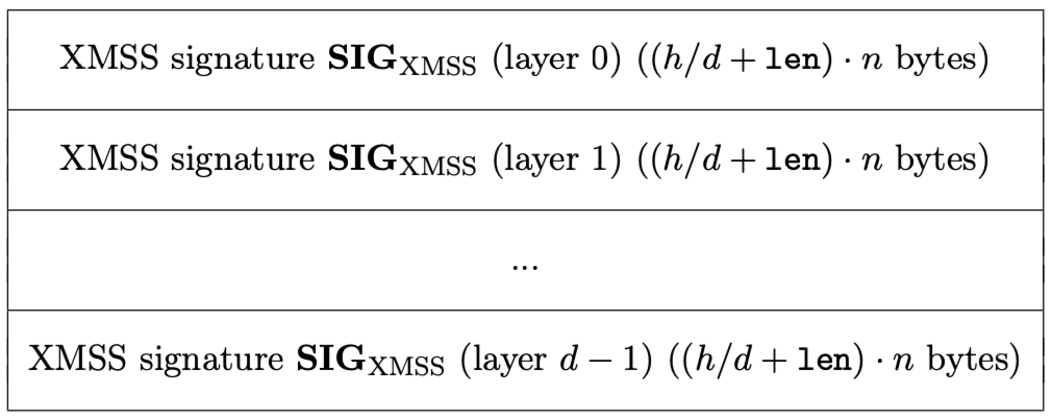
\includegraphics[width=.4\linewidth]{paper/spx-fig/Figure11.pdf}
    \caption{HT Signature.} \label{fig:spx11}
\end{figure}

\subsubsection{HT Signature Generation (Function \texttt{ht\_sign})}

To compute a HT signature $\sight$ of a message $M$, \texttt{ht\_sign} (\cref{alg:htsign}) uses \texttt{xmss\_sign} as defined in \cref{sec:xmsssign}. The algorithm \texttt{ht\_sign} takes as input a message $M$, a private seed \sk.\seed, a public seed $\pk.\seed$, and an index \texttt{idx}. The index identifies the leaf of the hypertree to be used to sign the message. The HT signature then consists of a stack of XMSS signatures using the XMSS trees on the path from the leaf with index idx to the top tree. Note that idx is passed as two separate arguments, split into an index to address the specific tree and the leaf index within that tree. This allows for a somewhat higher hypertree, as one can use a 64-bit integer for \texttt{tree\_idx} to support parameters that conform to $h<64+h_0$. This matches the parameters in this specification. If other parameter sets are used that allow greater $h$, the data type of \texttt{tree\_idx} MUST be adapted accordingly.

Algorithm \texttt{ht\_sign} uses \texttt{xmss\_pkFromSig} to compute the root node of an XMSS instance after that instance was used for signing. An alternative is to use \texttt{xmss\_PKgen}. However, \texttt{xmss\_PKgen} rebuilds the whole tree while \texttt{xmss\_pkFromSig} only does one call to \texttt{wots\_pkFromSig} and $(h_i-1)$ calls to $\hashH$ on layer $i$. The algorithm \texttt{ht\_sign} as described below is just one way to generate a HT signature. Other methods MAY be used as long as they generate the same output.

\begin{algorithm}
    \inputminted[breaklines,linenos,tabsize=2,mathescape,escapeinside=||]{C}{paper/code/ht_sign.cs}
    \caption{\texttt{ht\_sign} --- Generating an HT signature.}
    \label{alg:htsign}
\end{algorithm}

\subsubsection{HT Signature Verification (Function \texttt{ht\_verify})}

HT signature verification (\cref{alg:htverify}) can be summarized as $d$ calls to \texttt{xmss\_pkFromSig} and one comparison with a given value. HT signature verification takes a message $M$, a signature $\sight$, a public seed $\pk.\seed$, an index \texttt{idx} (split into a tree index and a leaf index, as above), and a HT public key $\pk_{\mathtt{HT}}.$

\begin{algorithm}
    \inputminted[breaklines,linenos,tabsize=2,mathescape,escapeinside=||]{C}{paper/code/ht_verify.cs}
    \caption{\texttt{ht\_verify} --- Verifying a HT signature $\bf {SIG}_{HT}$ on a message $M$ using a HT public key ${\bf PK}_{HT}$.}
    \label{alg:htverify}
\end{algorithm}
\section{BPORS+FP: Bucket-Thinned Few-Time Signatures}
\label{sec:bpors}

The \SPHINCSA\ hypertree HT is not used to sign the original message directly.
Instead, the randomized message hash selects a bottom HT leaf and gives an
$n$-byte digest \md.  Kylin signs this digest with BPORS+FP, a bucket-thinned
few-time signature component based on the construction in~\cite{bucketthinning}
and on forced-pruning style size control~\cite{EPRINT:AbrKat25}.  The resulting
BPORS+FP public key is then signed by the bottom XMSS tree of the hypertree.

BPORS+FP has an outer bucketing layer and a child PORS layer.  The outer layer
contains $K$ coordinates.  Each coordinate contains $2^B$ buckets, and each
bucket stores the public key of an independent child PORS instance.  A child
PORS instance has $t$ leaves and opens a $k$-subset of those leaves using the
Octopus authentication set of the left-filled Merkle tree on $t$ leaves.  Kylin
uses a global forced-pruning threshold $m_{\max}$: the signer repeats the
BPORS encoding hash with an explicit counter until the total authentication
node count, including the $KB$ outer authentication nodes and all child Octopus
nodes, is at most $m_{\max}$.

\subsection{BPORS+FP Parameters}
\label{sec:bporspara}

BPORS+FP uses the parameters $K,B,t,k,m_{\max}$ and a counter length
$c_{\mathrm{ctr}}$ in bytes:
\begin{itemize}
    \item $K$: the number of outer coordinates and selected child PORS keys.
    \item $B$: the bucket-address bit length; each coordinate has $2^B$ buckets.
    \item $t$: the number of leaves in each child PORS tree.  This value need
    not be a power of two; non-power-of-two trees use the left-filled tree
    convention.
    \item $k$: the number of leaves opened inside each selected child PORS key.
    \item $m_{\max}$: the fixed global authentication-node budget.
    \item $c_{\mathrm{ctr}}$: the number of bytes used to encode the rejection
    counter.  The packaged implementation uses $c_{\mathrm{ctr}}=8$.
\end{itemize}

For a digest \md and counter value $\mathtt{ctr}$, a domain-separated XOF maps
$(\md,\mathtt{ctr},\pk.\seed,\ADRS)$ to
\[
    ((j_0,I_0),\ldots,(j_{K-1},I_{K-1}))
    \in \left([2^B]\times\binom{[t]}{k}\right)^K .
\]
Here $j_c$ is the bucket selected in coordinate $c$, and
$I_c\subseteq[t]$ is the $k$-subset opened in the corresponding child tree.
The candidate is accepted when
\[
    A_{\mathrm{tot}}
    =KB+\sum_{c=0}^{K-1}\left|\operatorname{Oct}_t(I_c)\right|
    \le m_{\max}.
\]

\subsection{BPORS+FP Private Key and Public Key}

As with the rest of Kylin, BPORS+FP private values are generated
pseudorandomly from the single seed \sk.\seed.  The secret value for
coordinate $c$, bucket $j$, and child leaf $u$ is derived as
\[
    x_{c,j,u}\gets \PRF(\sk.\seed,\ADRS_{c,j,u}),
\]
where the address type and the coordinate, bucket, and child-leaf fields
separate this value from all WOTS and hypertree values.  The child leaf is
$\hashF(\pk.\seed,\ADRS_{c,j,u},x_{c,j,u})$.

Each child PORS public key is the root of the left-filled Merkle tree over its
$t$ child leaves.  For each outer coordinate $c$, the $2^B$ child public keys
are placed as leaves of a complete binary Merkle tree of height $B$.  The
BPORS+FP public key is
\[
    \pk_{\mathsf{BPORS}}
    =\Th_K(\pk.\seed,\ADRS_{\mathsf{BPORS\_PK}},
           \mathsf{root}_0\|\cdots\|\mathsf{root}_{K-1}),
\]
where $\mathsf{root}_c$ is the root of the outer tree for coordinate $c$.

\subsection{BPORS+FP Signature Generation}

A BPORS+FP signature contains the counter, the $Kk$ selected child secret
values, the child Octopus authentication nodes, the outer authentication
paths, and zero padding up to the fixed budget $m_{\max}$.  The signing
algorithm is shown in \cref{alg:bporpsign}.

\begin{algorithm}
    \inputminted[breaklines,linenos,tabsize=2,mathescape,escapeinside=||]{C}{paper/code/bpors_sign.cs}
    \caption{\texttt{bpors\_sign} --- Generate a BPORS+FP signature and public key.}
    \label{alg:bporpsign}
\end{algorithm}

\subsection{BPORS+FP Compute Public Key from Signature}

Kylin uses implicit verification for BPORS+FP.  Given \sigbpors and \md, the
verifier re-derives the accepted bucket labels and child subsets from the
counter, reconstructs each child public key from the revealed secrets and
Octopus nodes, reconstructs each outer root using the outer authentication
path, checks that unused authentication slots are zero, and finally compresses
the $K$ outer roots.  This is shown in \cref{alg:bporspkfromsig}.

\begin{algorithm}
    \inputminted[breaklines,linenos,tabsize=2,mathescape,escapeinside=||]{C}{paper/code/bpors_pkFromSig.cs}
    \caption{\texttt{bpors\_pkFromSig} --- Compute a BPORS+FP public key from a signature.}
    \label{alg:bporspkfromsig}
\end{algorithm}


\section{The Full Kylin Signature Scheme}
\label{sec:spx-core}
We now have all ingredients to describe our main construction \SPHINCSA.  It
keeps the SPHINCS-style hypertree structure, but uses \WOTSCS\ one-time
signatures and BPORS+FP as the bottom few-time signature component.

\subsection{\SPHINCSA\ Parameters}

\SPHINCSA\ has the following parameters:

\begin{itemize}

    \item $n$: the security parameter in bytes.

    \item $w$: the Winternitz parameter as defined in Section \ref{sec:wotspara}.
    
    \item $h$: the height of the hypertree as defined in Section \ref{sec:htpara}.
    
    \item $d$: the number of layers in the hypertree as defined in Section \ref{sec:htpara}.
    
    \item $K,B,t,k,m_{\max}$: the BPORS+FP parameters as defined in
    \cref{sec:bporspara}.
    
\end{itemize}

All the restrictions stated in the previous sections apply.  Moreover, from
these values the values $m$ and \wotslen are computed as

\begin{itemize}
    \item $m$: the message digest length in bytes. It is computed as
    $$
    m=n+\lfloor(h-h_0+7)/8\rfloor+\lfloor(h_0+7)/8\rfloor.
    $$
    The first $n$ bytes are the BPORS+FP digest.  The remaining bytes encode
    the hypertree tree and leaf indices.
    
    \item $\wotslen$: the number of $n$-byte string elements in a \WOTSCS\ private key, public key, and signature. The value $\wotslen$ is chosen so that the size of the following poset is larger than the desired message space $\bool^{8n}$ (cf.~\cref{sec:balanced wotsp}).
    \[\left| D_{ \wotslen, \lfloor \frac{\wotslen \cdot (w-1)}{2} \rfloor } \right| \geq 2^{8n} \enspace. \]

\end{itemize}
In the following, we assume that all algorithms have access to these parameters.

\subsection{\SPHINCSA\ Key Generation (Function \texttt{kylin\_keygen})}

The \SPHINCSA\ private key contains two elements. First, the $n$-byte secret seed $\sk.\seed$ which is used to generate all the \WOTSCS\ and BPORS+FP private key elements. Second, an $n$-byte PRF key $\sk.\prf$ which is used to deterministically generate a randomization value for the randomized message hash.

The \SPHINCSA\ public key also contains two elements. First, the HT public key, i.e.~the root of the tree on the top layer. Second, an $n$-byte public seed value $\pk.\seed$ which is sampled uniformly at random.

As \texttt{kylin\_sign} does not get the public key, but needs access to $\pk.\seed$ (and possibly to $\pk.\root$ for fault attack mitigation), the \SPHINCSA\ secret key contains a copy of the public key.

The description of algorithm \texttt{kylin\_keygen} assumes the existence of a function \texttt{sec\_rand} which on input $i$ returns $i$-bytes of cryptographically strong randomness.

\begin{algorithm}
    \inputminted[breaklines,linenos,tabsize=2,mathescape,escapeinside=||]{C}{paper/code/kylin_keygen.cs}
    \caption{\texttt{kylin\_keygen} ---  Generate a \SPHINCSA\ key pair.}
    \label{alg:spxkeygen}
\end{algorithm}

The format of a \SPHINCSA\ private and public key is given in \cref{fig:spx14}.

\begin{figure}[ht]
    \centering
    \begin{bytefield}[bitwidth=1.1em,bitheight=2em]{8}
        \wordbox{1}{$\sk.\mathtt{seed}$} \\
        \wordbox{1}{$\sk.\mathtt{prf}$} \\
        \wordbox{1}{$\pk.\mathtt{seed}$} \\
        \wordbox{1}{$\pk.\mathtt{root}$}
    \end{bytefield}
    \qquad
    \begin{bytefield}[bitwidth=1.1em,bitheight=2em]{8}
        \wordbox{1}{$\pk.\mathtt{seed}$} \\
        \wordbox{1}{$\pk.\mathtt{root}$}
    \end{bytefield} 

    %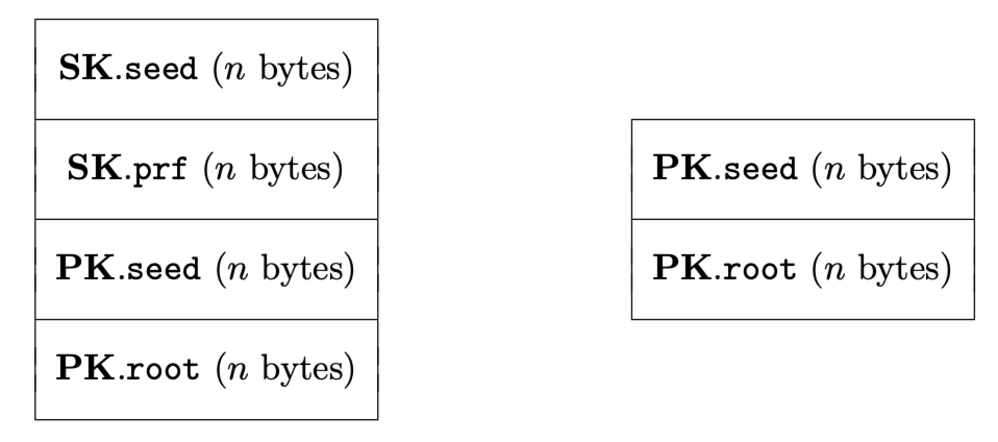
\includegraphics[width=.8\linewidth]{paper/spx-fig/Figure14.pdf}
    \caption{Left: \SPHINCSA\ secret key. Right: \SPHINCSA\ public key.} \label{fig:spx14}
\end{figure}

\subsection{\SPHINCSA\ Signature}

A \SPHINCSA\ signature $\sig$ is a byte string of length
\[
    n+c_{\mathrm{ctr}}+
    (Kk+m_{\max})n+(h+d\cdot\wotslen)n .
\]
It consists of an $n$-byte randomization string \randstr, a BPORS+FP signature
\sigbpors consisting of an explicit counter, $Kk$ $n$-byte secret values and
$m_{\max}$ $n$-byte authentication-node slots, and a HT signature $\sight$ of
$(h+d\cdot\wotslen)n$ bytes.

The data format for a signature is given in \cref{fig:spx15}.

\begin{figure}[ht]
    \centering
    \begin{bytefield}[bitwidth=1.1em,bitheight=2em]{16}
        \wordbox{1}{Randomness $\randstr$} \\
        \wordbox{1}{BPORS+FP Signature $\sigbpors$} \\
        \wordbox{1}{HT Signature $\sight$}
    \end{bytefield} 
    %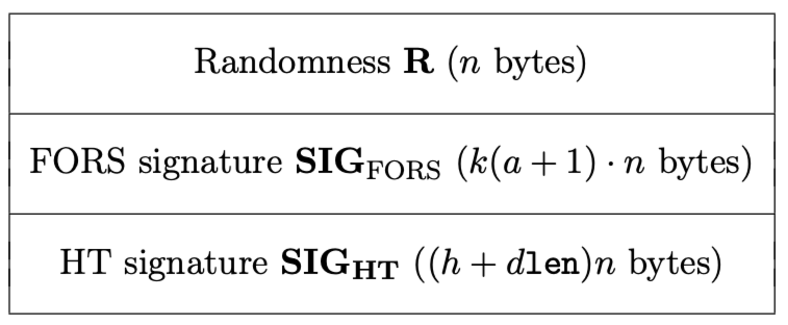
\includegraphics[width=.4\linewidth]{paper/spx-fig/Figure15.pdf}
    \caption{ \SPHINCSA\ signature.} \label{fig:spx15}
\end{figure}

\subsection{\SPHINCSA\ Signature Generation (Function \texttt{kylin\_sign})}

Generating a \SPHINCSA\ signature consists of four steps. First, a random value
\randstr is pseudorandomly generated. Next, this is used to compute an $m$ byte
message digest which is split into an $n$-byte BPORS+FP digest \md, a
$\lfloor(h-h_0+7)/8\rfloor$-byte tree index \texttt{tmp\_idx\_tree}, and a
$\lfloor(h_0+7)/8\rfloor$-byte leaf index \texttt{tmp\_idx\_leaf}.  The values
\texttt{idx\_tree} and \texttt{idx\_leaf} are computed by extracting the
necessary number of bits. The digest \md is then signed with the BPORS+FP key
pair associated with the \texttt{idx\_leaf}-th bottom leaf of the
\texttt{idx\_tree}-th XMSS tree on the lowest HT layer. The resulting
BPORS+FP public key is then signed using HT. The index is never actually used
as a whole, but immediately split into a tree index and a leaf index, for ease
of implementation.

When computing $\tt{R}$, the PRF takes a $n$-byte string opt which is initialized with $\pk.\seed$ but can be overwritten with randomness if the global variable \texttt{RANDOMIZE} is set. This option is given as otherwise \SPHINCSA\ signatures would be always deterministic.  

\begin{algorithm}[ht]
    \inputminted[breaklines,linenos,tabsize=2,mathescape,escapeinside=||]{C}{paper/code/kylin_sign.cs}
    \caption{ \texttt{kylin\_sign} --- Generating a \SPHINCSA\ signature.}
    \label{alg:spxsign}
\end{algorithm}

\subsection{\SPHINCSA\ Signature Verification (Function \texttt{kylin\_verify})}

\SPHINCSA\ signature verification (Algorithm \ref{alg:spxvrfy}) can be
summarized as recomputing the message digest and index, computing a candidate
BPORS+FP public key, and verifying the HT signature on that public key. Note
that the HT signature verification will fail if the BPORS+FP public key is not
matching the real one (with overwhelming probability). \SPHINCSA\ signature
verification takes a message $M$, a signature \sig, and a \SPHINCSA\ public
key $\pk$.

\begin{algorithm}[ht]
    \inputminted[breaklines,linenos,tabsize=2,mathescape,escapeinside=||]{C}{paper/code/kylin_verify.cs}
    \caption{ \texttt{kylin\_verify} --- Verify a \SPHINCSA\ signature $\bf SIG$ on a message $M$ using a \SPHINCSA\ public key $\bf PK$.}
    \label{alg:spxvrfy}
\end{algorithm}

\section{Parameter Sets and Hash/XOF Instantiation}
\label{sec:instantiations}

This section discusses instantiations for \SPHINCSA. \SPHINCSA\ can be viewed as a signature template. It is a way to build a signature scheme by instantiating the cryptographic function families used. We consider different ways to implement the cryptographic function families as different signature systems. Orthogonal to instantiating the cryptographic function families are parameter sets. Parameter sets assign specific values to the \SPHINCSA\ parameters described below.

In this section, we first define the requirements on parameters and discuss existing trade-offs between security, sizes, and speed controlled by the different parameters. Then we summarize the frozen NGCC-facing parameter sets and the hash/XOF instantiation used by the packaged implementation.


\subsection{\SPHINCSA\ Parameter Sets}

\SPHINCSA\ is described by the following parameters already described in the previous sections. All parameters take positive integer values.

\begin{itemize}

\item $n$: the security parameter in bytes.

\item $w$ : the Winternitz parameter.

\item $h$: the height of the hypertree.

\item $d$: the number of layers in the hypertree.

\item $K,B,t,k,m_{\max}$: the BPORS+FP few-time parameters.

\end{itemize}


Moreover, from these values the values $m$ and $\wotslen$ are computed as
\begin{itemize}
    \item $ m $: the message digest length in bytes. It is computed as
    $$m=n+\lfloor(h-h_0+7)/8\rfloor+\lfloor(h_0+7)/8\rfloor.$$
    \item $\wotslen$: the number of $n$-byte string elements in a \WOTSCS\ private key, public key, and signature.
    $$
    \wotslen = \min \left\{ \ell : \left| D_{\ell, \lfloor \frac{\ell \cdot (w-1)}{2} \rfloor} \right| \geq 2^{8n} \right\} \enspace,
    $$
    where the size of $D_{\ell, \lfloor \frac{\ell \cdot (w-1)}{2} \rfloor}$ is evaluated using the recurrence relation in \cref{equ:recurrence}.
\end{itemize}

We now repeat the roles of, requirements on, and properties of these parameters. Afterwards, we give several formulas that show their exact influence on performance and security. The security parameter $n$ is also the output length of all cryptographic function families besides $\hashmsg$. Therefore, it largely determines which security level a parameter set reaches. It is also the size of virtually any node within the \SPHINCSA\ structure and thereby also the size of all elements in a signature, i.e., the signature size is a multiple of $n$.

The Winternitz parameter $w$ determines the number and length of the hash chains per \WOTSCS\ instance. A greater value for $w$ linearly increases the length of the hash chains but logarithmically reduces their number. The number of hash chains exactly corresponds to the number of $n$-byte values in a \WOTSCS\ signature. Thereby it largely influences the size of a \SPHINCSA\ signature. The product of the number and the length of hash chains directly correlates with signing speed as essentially all time in HT signature generation is spent computing \WOTSCS\ public keys. Therefore, greater $w$ means shorter signatures but slower signing. However, note the exponential gap. The bigger $w$ gets, the more expensive is the signature size reduction. The Winternitz parameter does not influence \SPHINCSA\ security.

The height of the hypertree $h$ determines the number of bottom BPORS+FP
instances. Hence, it determines the probability that a bottom few-time key pair
is used several times, given the number of signatures made with a \SPHINCSA\
key pair. Hence, the height has a direct impact on security: A taller hypertree
gives more security. On the other hand, a taller tree leads to larger
signatures.

The number of layers $d$ is a pure performance trade-off parameter and does not influence security. It determines the number of layers of XMSS trees in the hypertree. The per-layer heights $(h_0,\ldots,h_{d-1})$ define the XMSS heights and must satisfy $\sum_{i=0}^{d-1} h_i = h$. Increasing $d$ usually allows smaller subtrees and faster signing. However, $d$ also controls the number of layers and thereby the number of \WOTSCS\ signatures within a HT and thereby a \SPHINCSA\ signature.

The parameters $K,B,t,k,m_{\max}$ determine the performance and security of
BPORS+FP.  Larger $B$ gives stronger bucket thinning because each child PORS key
sees a smaller fraction of the signing history, but it also increases the cost
of building the outer bucket trees and adds $KB$ outer authentication nodes.
Larger $K$ amplifies the cover-term exponent and opens more child keys.  The
child parameters $t$ and $k$ determine the PORS cover term and the size of each
child opening.  The threshold $m_{\max}$ fixes the authentication-node payload:
smaller values reduce signatures but increase the expected number of counter
trials.

The message digest length $m$ is the output length of $\hashmsg$ in bytes. It
is $n+\lfloor(h-h_0+7)/8\rfloor+\lfloor(h_0+7)/8\rfloor$ bytes.

The number $\wotslen$ of chains in a \WOTSCS\ key pair determines the \WOTSCS\ signature size.

\subsubsection{Influence of Parameters on Security and Performance} \label{sec:securityandperformance}

In the following we provide formulas to compute speed, size and security for a given \SPHINCSA\ parameter set. This supports parameter selection. We also provide a SAGE script in Appendix \ref{apx:script}.
 

\paragraph{Key Generation.} 
Generating the \SPHINCSA\ private key and $\pk.\seed$ requires three calls to a secure random number generator. Next we have to generate the top tree (layer $d-1$). For the leaves we need to do $2^{h_{d-1}}$ \WOTSCS key generations ($\wotslen$ calls to PRF for generating the $\sk$ and $w \wotslen$ calls to $\hashF$ for the $\pk$) and we have to compress the \WOTSCS\ public key (one call to $\Th_{\wotslen}$). Computing the root of the top tree requires $(2^{h_{d-1}}-1)$ calls to $\hashH$.

\paragraph{Signing.}
For randomization and message compression we need one call to $\PRFmsg$, and
one to $\hashmsg$.  The BPORS+FP signing cost consists of counter trials,
generation of the $Kk$ revealed child secrets, construction of the selected
child openings, and construction of the $K$ outer authentication paths.  In the
packaged implementation this is dominated by constructing the selected outer
bucket trees, i.e., about $K\cdot 2^B$ child roots, each over $t$ child leaves,
plus the child-opening work for the selected buckets.  Next, we compute one HT
signature which consists of $d$ trees similar to the key generation. Hence, we
have to do $\sum_{i=0}^{d-1} 2^{h_i}$ times $\wotslen$ calls to $\PRF$ and
$w \wotslen$ calls to $\hashF$ as well as $\sum_{i=0}^{d-1} 2^{h_i}$ calls to
$\Th_{\wotslen}$. For computing the root of each tree we get additionally
$\sum_{i=0}^{d-1} (2^{h_i}-1)$ calls to $\hashH$.

\paragraph{Verification.}
First we need to compute the message hash using $\hashmsg$. We need to do one
BPORS+FP public-key reconstruction.  This requires $Kk$ calls to $\hashF$ to
hash the revealed child secrets into leaves, one child-tree reconstruction for
each selected coordinate using the supplied Octopus nodes, $KB$ calls to
$\hashH$ for the outer authentication paths, and one call to $\Th_K$ for
hashing the outer roots. Next, we have to verify $d$ XMSS signatures which
takes $< w \wotslen$ calls to $\hashF$ and one call to $\Th_{\wotslen}$ each
for \WOTSCS\ signature verification\footnotemark. It also needs
$\sum_{i=0}^{d-1} h_i = h$ calls to $\hashH$ for the $d$ root computations.

\footnotetext{It should be noted that the $w \wotslen$ bound for calls to $\hashF$ is a worst-case bound. This is a bound on the cost for \WOTSCS signature verification. Given that the messages are hash values which can be assumed to be close to uniformly distributed, this value will be closer to the average-case bound $(w/2)\wotslen$ in actual measurements.}

The size of the \SPHINCSA\ private and public keys along with the signature are
$4n$, $2n$, and
\[
    n+c_{\mathrm{ctr}}+(Kk+m_{\max})n+(h+d\cdot\wotslen)n
\]
respectively.

The classical and quantum generic-security proxies are computed from the
BPORS+FP cover term in \cref{sec:proof-concrete}; small constant factors inside
the logarithm are neglected.



\subsubsection{Proposed Parameter Sets and Security Levels}

As explained in the previous subsection, even for a fixed security level the design of \SPHINCSA\ supports different tradeoffs between signature size and speed. For this submission package, we use the three NGCC-aligned Kylin instances listed in \cref{tab:ngcc-parameters}. These instances are generated by the repository-local parameter script and tuned to meet the legacy $127/255/511$ classical generic-security thresholds together with the corresponding quantum-security proxies.

\begin{table}[H]
    \centering
    \caption{Frozen NGCC-aligned Kylin parameter families used by the packaged primary implementations.}
    \label{tab:ngcc-parameters}
    \scriptsize
    \resizebox{\linewidth}{!}{%
\begin{tabular}{l c c c c l c c c c c c c}
    \toprule
    Family & NGCC lvl & $q$ & $n$ & $h/d$ & $(h_0,\ldots,h_{d-1})$ & $(K,B,t,k,m_{\max})$ & $w$ & $\wotslen$ & bitsec & pk & sk & sig \\ \midrule
    Kylin-128 & 128/80 & $2^{64}$ & 16 & 62/7 & $(8,9,9,9,9,9,9)$ & $(4,7,128,6,95)$ & 17 & 33 & 127.055 & 32 & 64 & 6616 \\
    Kylin-256 & 256/128 & $2^{64}$ & 32 & 65/8 & $(8,8,8,8,8,8,8,9)$ & $(9,8,66,5,187)$ & 16 & 66 & 255.156 & 64 & 128 & 26440 \\
    Kylin-512 & 512/256 & $2^{64}$ & 64 & 64/8 & $(8,8,8,8,8,8,8,8)$ & $(14,8,256,5,415)$ & 43 & 96 & 511.663 & 128 & 256 & 84360 \\
    \bottomrule
    \end{tabular}%
    }
\end{table}


\subsection{Instantiations of Hash Functions} \label{sec:hashfunctions}

For the NGCC submission package, hash and XOF calls follow the ICCS auxiliary
interface used by the bundled implementation code. In particular, the current
package uses \texttt{sm3hash}, \texttt{pseudohash}, and \texttt{pseudoXOF}, with
domain-separated wrappers built on top of \texttt{pseudoXOF} in the
\texttt{hash\_iccs.c} and \texttt{thash\_iccs.c} modules.

Recall that $n$ and $m$ are the security parameter and the message-digest
length in bytes.

The implementation-level mapping is summarized as follows:
\begin{align*}
    \hashmsg (\randstr, \pk.\seed, \pk.\root, M)
        &= \mathrm{pseudoXOF}(\mathtt{tag}_{H\_msg} \| \randstr \| \pk.\seed \| \pk.\root \| M, m),\\
    \PRF(\pk.\seed, \sk.\seed, \ADRS)
        &= \mathrm{pseudoXOF}(\mathtt{tag}_{PRF} \| \pk.\seed \| \ADRS \| \sk.\seed, n),\\
    \PRFmsg(\sk.\prf, \mathtt{OptRand}, M)
        &= \mathrm{pseudoXOF}(\mathtt{tag}_{PRFmsg} \| \sk.\prf \| \mathtt{OptRand} \| M, n),\\
    \hashF(\pk.\seed, \ADRS, M_1)
        &= \mathrm{pseudoXOF}(\mathtt{tag}_{F} \| \pk.\seed \| \ADRS \| M_1, n),\\
    \hashH(\pk.\seed, \ADRS, M_1 \| M_2)
        &= \mathrm{pseudoXOF}(\mathtt{tag}_{H} \| \pk.\seed \| \ADRS \| M_1 \| M_2, n),\\
    \Th_\ell(\pk.\seed, \ADRS, M)
        &= \mathrm{pseudoXOF}(\mathtt{tag}_{T} \| \pk.\seed \| \ADRS \| M, n).
\end{align*}

Here, \texttt{sm3hash} is the fixed-output SM3 interface and
\texttt{pseudohash}/\texttt{pseudoXOF} provide the variable-length hash and XOF
behavior required by the NGCC API profile. The public packaged implementation
uses explicit domain-separation tags for these calls and keeps the
address/seed layout aligned with the ICCS helper functions.
